\section{Circuito analógico de entrada\label{testcircuito}}

La caracterización del circuito de entrada serán básicas puesto que existe un gran número de referencias y de opciones que se pueden comprar a un precio reducido ya montadas. El montaje del módulo para este proyecto ha surgido únicamente de la curiosidad académica y no de conveniencia técnica.

\subsection{Saturación y dependencia con la tensión de entrada}
Es necesario tener en cuenta que para realizar todas las medidas que se presentan a continuación ha sido necesario generar dos señales de entrada para el circuito. No hay que olvidar que al tratarse de una entrada balanceada, se debe introducir un señal en un canal y otra duplicada pero en contrafase en el otro. Afortunadamente, el generador de funciones disponible en laboratorio ofrece esta posibilidad únicamente pulsando un botón. En lo sucesivo, cuando me refiero a la señal de entrada siempre me referiré al conjunto de la señal en cuestión más el duplicado en contrafase.

En este apartado se pretende caracterizar la respuesta del circuito frente a entradas de diferentes tensiones, utilizando diferentes posiciones del potenciómetro y permitiendo hallar el punto de saturación del conjunto para una entrada sinusoidal. Las medidas tomadas son las mostradas en la tabla siguiente.\\

\begin{table}[htb]
\centering
\begin{tabular}{|c |c |c |c |c |c|}
%%%%%%%%%%%%%%%%%%%%%%%%%%%%%%%%%%%%%%%%%%%%%%%%%%%%%%%%%%%%%%%%%%%%%%%%%%%%%%%%%%%%%%%%%%%%%%%%%%%%%%%%%%%%%%%
\hline
$V_{in}(mV)$            &$Pos.~Pot.$   &$V_{out}(mV)$          &$~~~~G (V)~~~~$      &$~~G (dB)~~$     &$Rango~Pot.(dB)$   \\
\hline
\multirow{2}{1.5cm}{\centering{518,8}} & Min. & 365,6 &  0.7047 & -3,04 & \multirow{2}{1.5cm}{\centering{8,12}} \\
                                      & Max. & 931,3 &  1,7951 & 5,08 &                                       \\ \hline
\multirow{2}{1.5cm}{\centering{1018}} & Min. & 643,8 &  0,6319 & -3,99 & \multirow{2}{1.5cm}{\centering{12,05}} \\
                                      & Max. & 2578 &  2,5304 & 8,06 &                                       \\ \hline
\multirow{2}{1.5cm}{\centering{2016}} & Min. & 1243 &  0,6170 & -4,19 & \multirow{2}{1.5cm}{\centering{9,10}} \\
                                      & Max. & 3547 &  1,7594 & 4,91 &                                       \\ \hline
\multirow{2}{1.5cm}{\centering{3313}} & Min. & 1875 &  0,5660 & -4,94 & \multirow{2}{1.5cm}{\centering{9.59}} \\
                                      & Max. & 5656 &  1,7072 & 4,65 &                                       \\ \hline           
\end{tabular}
%\caption{\label{tabla:sat_medidas}Relación de tiempo de trabajo destinado a cada ámbito.}
\end{table}

En esta tabla, la columna \emph{Pos. Pot} hace referencia la posición del potenciómetro, es decir, si estaba ajustado al mínimo o al máximo, lo que permite estimar el rango de la ganancia en la columna \emph{Rango. Pot}. Se puede apreciar como la mayor sensibilidad se obtiene para la entrada de $1V_{pp}$ aproximadamente. La última medida corresponde al punto de saturación, el cual se ha obtenido empíricamente aumentando la tensión de entrada hasta que se observase recorte en la salida (con ganancia máxima), el proceso se muestra en la figura \ref{fig:medsat}.

\begin{figure}[!hbt]
\begin{center}
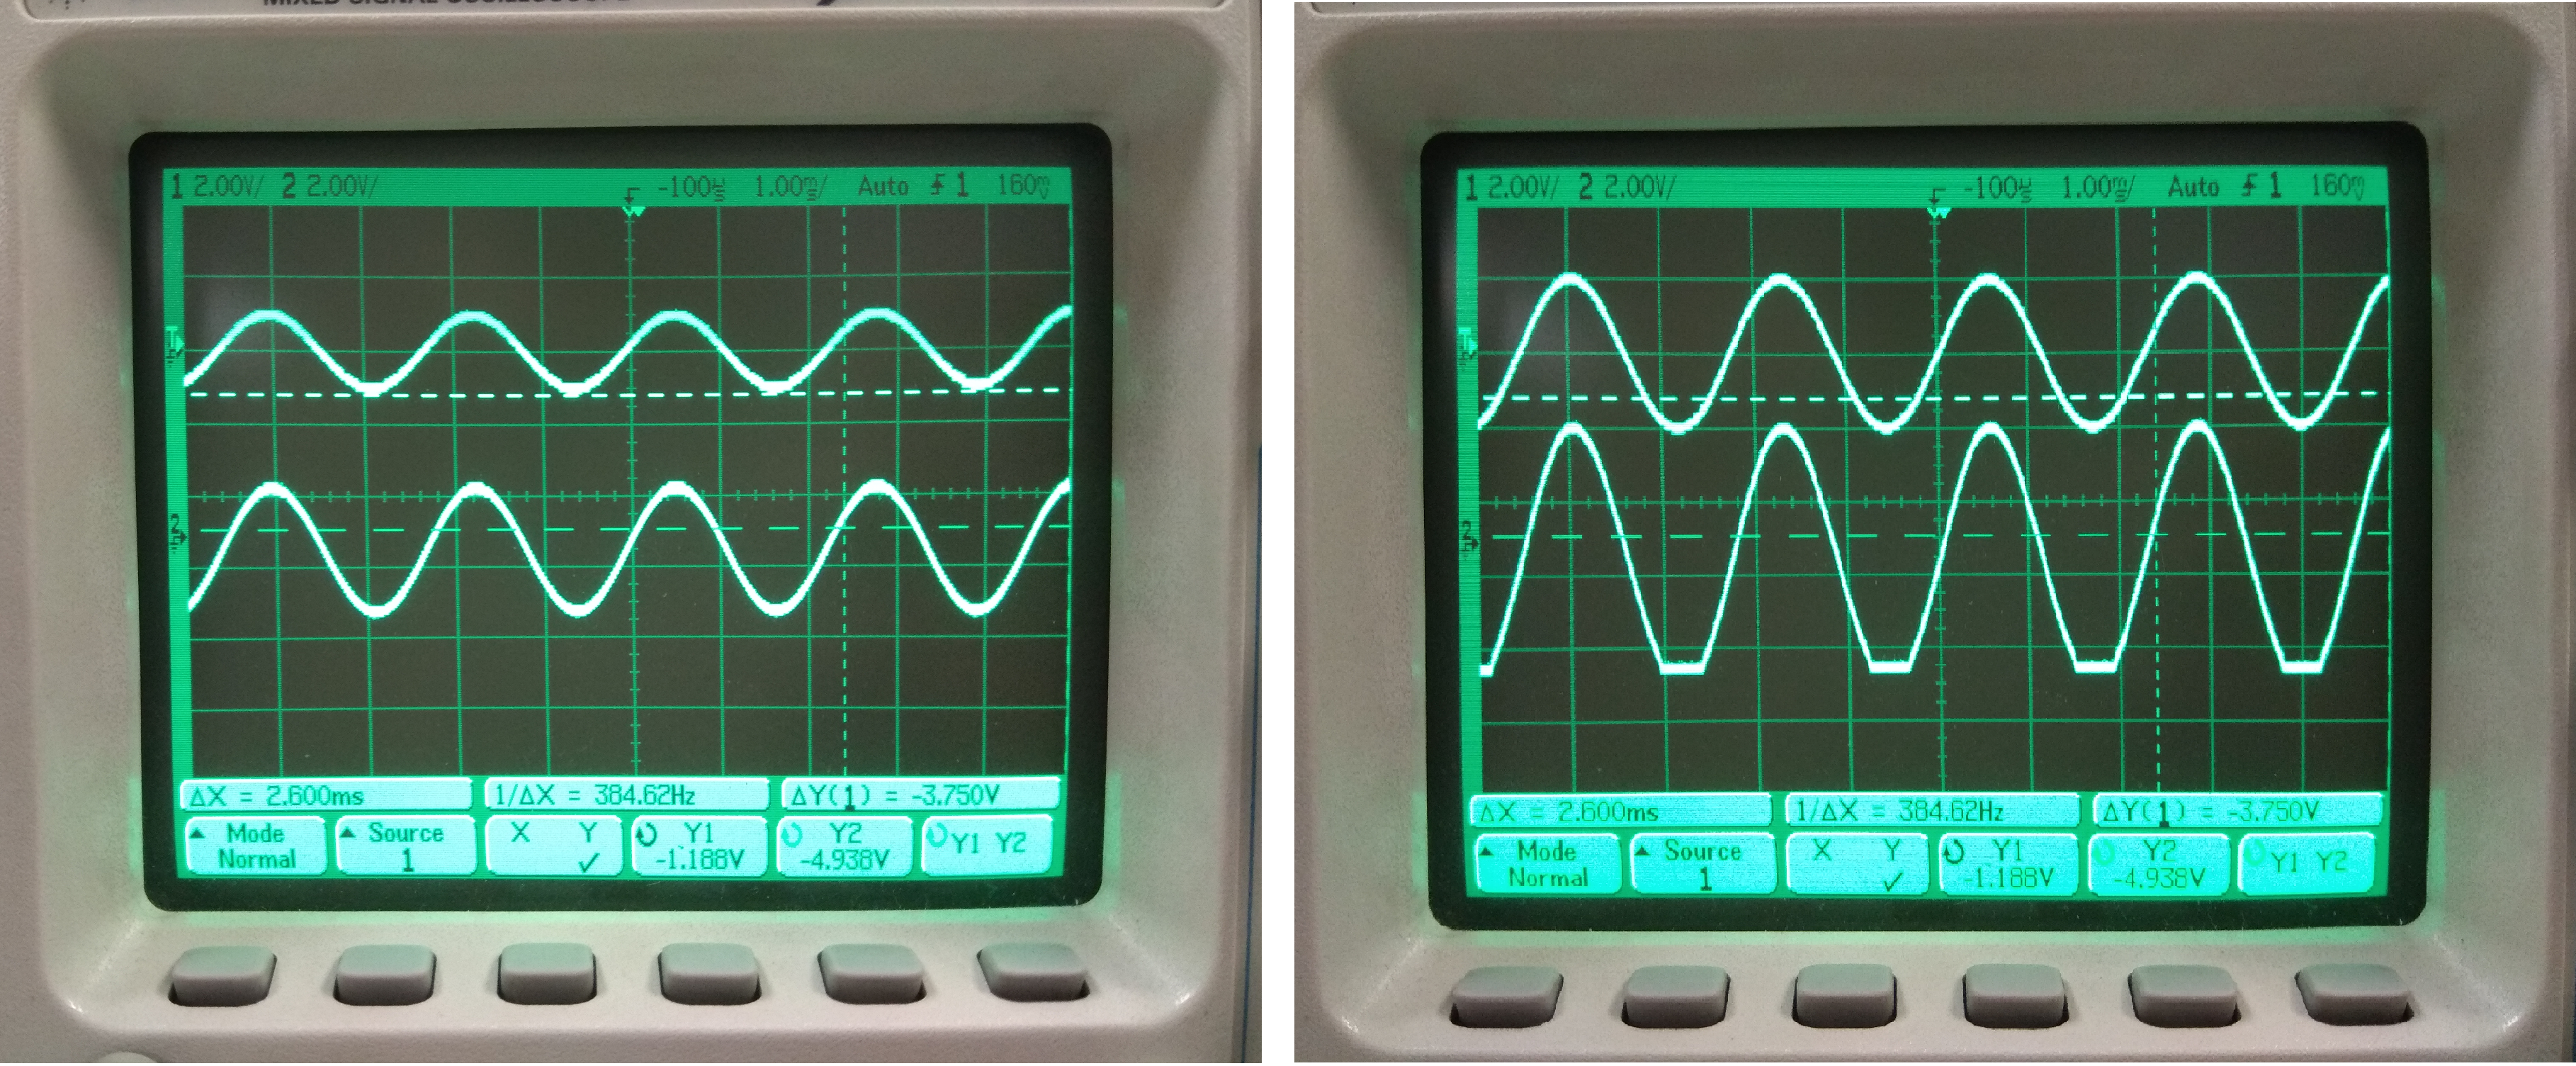
\includegraphics[width=12cm]{img/medsat.png}
\caption{\label{fig:medsat}Fotografías de las medidas realizadas buscando el punto de saturación}
\end{center}
\end{figure}

\subsection{Dependencia de la ganancia con la frecuencia}
\subsection{Otros parámetros}
\section{Algoritmo de \emph{Vocoder de fase}}

Para probar el algoritmo que se va a implementar se ha utilizado un fragmento breve interpretado con saxofón alto del tema \emph{Billie's Bounce} de \emph{Charlie Parker}. La grabación de este fragmento está realizada con un micrófono corriente no profesional y se ha guardado en formato \emph{.wav}, es decir, sin compresión. Este formato, al igual que Matlab utiliza una frecuencia de muestro $F_{s} = 44.1~kHz$.

El fichero de prueba se encuentra en el Apéndice \ref{ap:pruebaalgoritmo}. Esta función precisa de una ruta de archivo de audio que se va a octavar y de un entero que se corresponde con un cierto número de muestras de retraso. Este último parámetro permite cuantificar los efectos de la latencia en la FPGA.

\begin{figure}[hbt]
\begin{center}
\includegraphics[width=15cm]{img/testAlFreq.png}
\caption{\label{fig:testFreq}Suma de las componentes en frecuencia}
\end{center}
\end{figure}

El resultado de la prueba son dos archivos de audio: uno contiene el fichero de entrada octavado y el otro mezcla la entrada con el fichero octavado en una proporción de 35\% y 65\% respectivamente. Lógicamente, es en este último en el que la latencia tiene efecto. Adicionalmente se ha graficado tanto la suma de las componentes en frecuencia (figura~\ref{fig:testFreq}) como en el dominio del tiempo (figura~\ref{fig:testTime}) ambos con latencia nula. En la primera podemos observar claramente como los picos se encuentran en frecuencias de la mitad de valor debido a la octavación. Aunque pueda parecer que el resultado muestra la serie armónica, hay que recordar que en este fragmento se han interpretado múltiples notas, cada una con sus correspondientes frecuencias y armónicos asociados, por lo que la similitud que vemos entre esta gráfica y la serie armónica se debe a que las notas de la serie se utilizan más frecuentemente en la melodía. 

\begin{figure}[!bht]
\begin{center}
\includegraphics[width=15cm]{img/testAlTime.png}
\caption{\label{fig:testTime}Comparativa de los ficheros resultantes}
\end{center}
\end{figure}

En la gráfica correspondiente al dominio del tiempo se observa una ligera pérdida de amplitud en la señal debido al procesado. Para cuantificar el valor de estas pérdidas se utiliza el cociente entre el valor medio de la señal de salida entre el de la entrada, resultando en \textbf{1,5586 dB} para la señal octavada y \textbf{2,3890 dB} para la mezcla de ambas. También se puede apreciar como la forma de onda no se ha distorsionado en exceso; la calidad del audio resultante resulta razonablemente buena teniendo en cuenta que se ha pretendido simular el comportamiento de la FPGA con una longitud de transformada de 512 muestras de 16 bit.
[UNA VEZ HALLADA LA LATENCIA DE LA FPGA, INTRODUCIR ESE VALOR EN MATLAB Y COMPARAR]

\section{Sobre la implementación en FPGA}